\PassOptionsToPackage{
  usenames,
  fixpdftex,
  dvipsnames,
  svgnames,
  x11names
}{xcolor}
\PassOptionsToPackage{
  font=small,
  labelfont=bf,
  labelsep=period,
  justification=RaggedRight,
  format=plain,
  singlelinecheck=off
}{caption}
\PassOptionsToPackage{hyphens}{url}

\documentclass[
  oneside,
  openany,
  numbers=noendperiod,
  parskip=half,
  bibliography=totoc
]{scrbook}\usepackage[]{graphicx}\usepackage{xcolor}
%% maxwidth is the original width if it is less than linewidth
%% otherwise use linewidth (to make sure the graphics do not exceed the margin)
\makeatletter
\def\maxwidth{ %
  \ifdim\Gin@nat@width>\linewidth
    \linewidth
  \else
    \Gin@nat@width
  \fi
}
\makeatother

\definecolor{fgcolor}{rgb}{0.345, 0.345, 0.345}
\newcommand{\hlnum}[1]{\textcolor[rgb]{0.686,0.059,0.569}{#1}}%
\newcommand{\hlstr}[1]{\textcolor[rgb]{0.192,0.494,0.8}{#1}}%
\newcommand{\hlcom}[1]{\textcolor[rgb]{0.678,0.584,0.686}{\textit{#1}}}%
\newcommand{\hlopt}[1]{\textcolor[rgb]{0,0,0}{#1}}%
\newcommand{\hlstd}[1]{\textcolor[rgb]{0.345,0.345,0.345}{#1}}%
\newcommand{\hlkwa}[1]{\textcolor[rgb]{0.161,0.373,0.58}{\textbf{#1}}}%
\newcommand{\hlkwb}[1]{\textcolor[rgb]{0.69,0.353,0.396}{#1}}%
\newcommand{\hlkwc}[1]{\textcolor[rgb]{0.333,0.667,0.333}{#1}}%
\newcommand{\hlkwd}[1]{\textcolor[rgb]{0.737,0.353,0.396}{\textbf{#1}}}%
\let\hlipl\hlkwb

\usepackage{framed}
\makeatletter
\newenvironment{kframe}{%
 \def\at@end@of@kframe{}%
 \ifinner\ifhmode%
  \def\at@end@of@kframe{\end{minipage}}%
  \begin{minipage}{\columnwidth}%
 \fi\fi%
 \def\FrameCommand##1{\hskip\@totalleftmargin \hskip-\fboxsep
 \colorbox{shadecolor}{##1}\hskip-\fboxsep
     % There is no \\@totalrightmargin, so:
     \hskip-\linewidth \hskip-\@totalleftmargin \hskip\columnwidth}%
 \MakeFramed {\advance\hsize-\width
   \@totalleftmargin\z@ \linewidth\hsize
   \@setminipage}}%
 {\par\unskip\endMakeFramed%
 \at@end@of@kframe}
\makeatother

\definecolor{shadecolor}{rgb}{.97, .97, .97}
\definecolor{messagecolor}{rgb}{0, 0, 0}
\definecolor{warningcolor}{rgb}{1, 0, 1}
\definecolor{errorcolor}{rgb}{1, 0, 0}
\newenvironment{knitrout}{}{} % an empty environment to be redefined in TeX

\usepackage{alltt}

% Page layout
\usepackage[
  a4paper,
  left=23mm,
  top=27.4mm,
  bottom=27.4mm,
  %headsep=2\baselineskip,
  textwidth=107mm,
  marginparsep=8mm,
  marginparwidth=49mm,
  %textheight=49\baselineskip,
  %headheight=\baselineskip
]{geometry}

\usepackage{multicol}

\usepackage{marginfix}
%\usepackage{morefloats}

% Headers and footers
\usepackage[%
  automark,
  headsepline=false,
  headwidth=textwithmarginpar,
  footwidth=head
]{scrlayer-scrpage}

\clearpairofpagestyles
\rofoot[\pagemark]{\pagemark}
\lohead{\headmark}

% Title page
\title{eulerr: Area-Proportional Euler Diagrams with Ellipses}
\author{Johan larsson}
\date{\today}

\renewcommand{\maketitle}{%
  \cleardoublepage
  \begin{addmargin*}[0.25\overhang]{-0.75\overhang}%
    \centering
    \vspace*{2cm}
    
\includegraphics[width=0.3\textwidth]{LundUniversity_C2line_BLACK}\par\vspace{1cm}
    \vspace{0.5cm}
    {\scshape\Large Bachelor Thesis \par}
    {\Huge\bfseries eulerr: Area-Proportional Euler Diagrams with Ellipses \par}
    \vspace{2cm}
    {\huge\itshape Johan Larsson \par}
    \vspace{2cm}
    {\Large{\itshape supervised by}\par Peter Gustafsson}
    \vfill
    {\Large \today\par}
    \vfill
    {\large \itshape Submitted in partial fulfillment of the requirements for the degree of\\
      Bachelor of Science in Statistics\\
      at the Department of Statistics, Lund University}
  \end{addmargin*}%
  \thispagestyle{empty}
}

\usepackage[font=footnotesize]{subcaption}
\usepackage{graphicx}
\usepackage{booktabs}
\usepackage[document]{ragged2e}
\usepackage[shortlabels]{enumitem}
\usepackage[noend]{algpseudocode}
\usepackage{etoolbox}
%\usepackage[swedish]{babel}
\usepackage[square,numbers,sort&compress]{natbib}
\usepackage{floatrow}
\usepackage{environ}
\usepackage{xspace}

% Fonts
\usepackage[utf8]{inputenc}
\usepackage[T1]{fontenc}
\usepackage[lining]{libertine}
\usepackage{textcomp}
\usepackage[varqu,varl,scaled=0.93]{inconsolata}
\usepackage{mathtools}
\usepackage{amsthm}
\usepackage[libertine,vvarbb,libaltvw,liby]{newtxmath}
\usepackage[scr=rsfso]{mathalfa}
\usepackage{bm}
\useosf
\usepackage{microtype}

% Two-column bibliography
\patchcmd{\thebibliography}{\list}{\begin{multicols}{2}\small\list}{}{}
\appto{\endthebibliography}{\end{multicols}}

% Block margins for caption around figure and table environments
\BeforeBeginEnvironment{figure}{\blockmargin}
\AfterEndEnvironment{figure}{\unblockmargin}
\BeforeBeginEnvironment{table}{\blockmargin}
\AfterEndEnvironment{table}{\unblockmargin}

% Floats
\DeclareNewFloatType{algorithm}{fileext=alg, name=Algorithm}
\DeclareFloatSeparators{marginparsep}{\hskip\marginparsep}
\floatsetup[figure]{%
  margins=hangright,
  capposition=beside,
  capbesidesep=marginparsep,
  capbesideposition={top,right},
  floatwidth=\textwidth}
\floatsetup[table]{%
  margins=hangright,
  capposition=beside,
  capbesidesep=marginparsep,
  capbesideposition={top,right},
  floatwidth=\textwidth}
\floatsetup[widefigure]{%
  margins=hangright,
  capposition=bottom}
\floatsetup[widetable]{%
  margins=hangright,
  capposition=top}
\floatsetup[algorithm]{%
  margins=hangright,
  capposition=beside,
  capbesidesep=marginparsep,
  capbesideposition={top,right},
  floatwidth=\textwidth}
\captionsetup[subfigure]{position=b,justification=RaggedRight}
\captionsetup[sub]{justification=RaggedRight}

% Provide marginfigure
\NewEnviron{marginfigure}{%
  \marginpar{%
    \captionsetup{type=figure}
    \BODY
  }%
}

% Graphics options
\setkeys{Gin}{%
  width=\linewidth,
  totalheight=\textheight,
  keepaspectratio
}
\graphicspath{{graphics/}}

% Extended verbatim environments
\usepackage{fancyvrb}
\fvset{fontsize=\small}% default font size for fancy-verbatim environments

% Provide fullwidth environment
\newlength{\overhang}
\setlength{\overhang}{\marginparwidth}
\addtolength{\overhang}{\marginparsep}

\newenvironment{fullwidth}{%
  \blockmargin
  \begin{addmargin*}[0em]{-\overhang}%
}{%
  \end{addmargin*}%
  \unblockmargin
}

\newcommand{\proglang}[1]{\textsf{#1}}
\newcommand{\pkg}[1]{{\fontseries{b}\selectfont #1}}
\newcommand{\code}[1]{\texttt{#1}}

% Custom operators
\DeclareMathOperator{\E}{E}
\DeclareMathOperator{\Pois}{Pois}
\DeclareMathOperator{\B}{Bin}
\DeclareMathOperator{\V}{Var}
\DeclareMathOperator{\Exp}{Exp}

% Cross-referencing and colors
\usepackage{hyperref}
\usepackage[noabbrev,capitalize,nameinlink]{cleveref}
\usepackage{xcolor}
\hypersetup{%
  linkcolor=SteelBlue4,
  citecolor=SteelBlue4,
  urlcolor=SteelBlue4,
  colorlinks=true,
  breaklinks=true
}

% Theorems
\newtheorem{mydef}{Definition}[chapter]

% Redefine footnotes to be marginnotes
\newcounter{snmark}
\setcounter{snmark}{0}

\newcommand*{\makesidenotemark}{\/\textsuperscript{\thesnmark}}

\renewcommand{\footnote}[1]{%
  \refstepcounter{snmark}%
  \makesidenotemark{}%
  \marginpar{\RaggedRight\small\textsuperscript{\thesnmark}\,#1}%
}

% Add cref
\newcommand{\secref}[1]{\hyperref[#1]{\ref*{#1}~\nameref*{#1}}}

% Fix vdots and ddots for smallmatrix
\newcommand{\svdots}{\raisebox{3pt}{$\scalebox{.75}{\vdots}$}}
\newcommand{\sddots}{\raisebox{3pt}{$\scalebox{.75}{$\ddots$}$}}

\let\ts\textsuperscript

% Rotate text 90 degrees (for table)
\newcommand*\rot{\rotatebox{90}}

% Libertine in tabular
\makeatletter
\AtBeginDocument{\def\libertine@figurealign{}\libertineOsF}
\newcommand\libertineTabular{\def\libertine@figurealign{T}\libertineLF}
\makeatother
\AtBeginEnvironment{tabular}{\libertineTabular}

% Do while loop
\algdef{SE}[DOWHILE]{Do}{DoWhile}{\algorithmicdo}[1]{\algorithmicwhile\ #1}%
\algnewcommand\And{\textbf{and}\xspace}
\algnewcommand\Or{\textbf{or}\xspace}
\algnewcommand\All{\textbf{all}\xspace}
\IfFileExists{upquote.sty}{\usepackage{upquote}}{}
\begin{document}



\frontmatter
\maketitle

\begin{addmargin*}[0.5\overhang]{-0.5\overhang}
{\hypersetup{linkcolor=black}
\tableofcontents
}

\chapter*{Abstract}
\addcontentsline{toc}{chapter}{Abstract}

Euler diagrams are common and intuitive visualizations for data involving
sets and relationships thereof. Compared to Venn diagrams, Euler diagrams do not
require all set relationships to be present and may therefore be area-proportional
also with subset or disjoint relationships in the input.
Most Euler diagrams use circles, but circles do not always
support accurate diagrams. A promising alternative for Euler diagrams is ellipses,
which, in theory,enable accurate diagrams for a wider range
of input. Ellipses, however, have not yet
been implemented for more than three sets or three-set diagrams where
there are disjoint or subset relationships. The aim of this thesis is
to present a method and software for elliptical Euler diagrams for any
number of sets.

In this thesis, we provide and outline an R-based implementation called eulerr.
It fits Euler diagrams using numerical optimization and exact-area
algorithms through two steps: first, an initial layout is formed using
the sets' pairwise relationships; second, this layout is finalized
taking all the sets' intersections into account.

Finally, we compare eulerr with other software implementations of Euler
diagrams and show that the package
is overall both more consistent and accurate as well as
faster for up to seven sets compared to the other R-packages. eulerr perfectly
reproduces samples of circular Euler diagrams as well
as three-set diagrams with ellipses, but performs suboptimally with elliptical
diagrams of more than three sets. eulerr also outperforms the other software tested in
this thesis in fitting Euler diagrams to set configurations that might
lack exact solutions provided that we use ellipses; eulerr's circular diagrams,
meanwhile, fit better
on all accounts save for the diagError metric in the case of three-set diagrams.

\par\noindent\rule{\textwidth}{0.5pt}
\itshape\noindent\textbf{Keywords:} Euler diagrams, Venn diagrams, ellipses, R,
computer graphics, area-proportional, software

\end{addmargin*}
\mainmatter

\chapter{Introduction}

\section{Background}
\label{sec:background}

% Data visualizations represent one of the most intuitive forms of data
% presentation. Because they work on multiple dimensions, they possess the
% potential to convey intricate relationships that single statistics or tables
% never can.

Visual displays of data make for clear and compelling presentations,
utilizing multiple dimensions to inform concisely and intuitively.
Compared to tables and text,
visualization possess the potential to convey even intricate relationships with
effective use of ink.

Data visualizations, however, are only effective when they illustrate
relationships. Consider, for instance, a disc labelled
\emph{Men}\footnote{%
\begin{knitrout}\small
\definecolor{shadecolor}{rgb}{0.969, 0.969, 0.969}\color{fgcolor}

\includegraphics[width=\maxwidth]{figure/men-1} \hfill{}



\end{knitrout}
}---it says nothing by itself; yet if we juxtapose it with another, smaller, disc
labelled \emph{Children}\footnote{%
\begin{knitrout}\small
\definecolor{shadecolor}{rgb}{0.969, 0.969, 0.969}\color{fgcolor}

\includegraphics[width=\maxwidth]{figure/children-1} \hfill{}



\end{knitrout}
}, the graphic starts to become informative, now displaying the relative sizes
of two sets. If next we intersect the two
discs, producing an overlap\footnote{%
\begin{knitrout}\small
\definecolor{shadecolor}{rgb}{0.969, 0.969, 0.969}\color{fgcolor}

\includegraphics[width=\maxwidth]{figure/childrenMen-1} \hfill{}



\end{knitrout}
}, we successfully visualize the
relative proportions of men and children, as well as their intersection. The diagram
we have constructed is an \emph{Euler diagram}.

The Euler diagram, originally proposed by Leonard Euler in
1802~\citep{Euler_1802}, is
a generalization of the obiquiteous \emph{Venn diagram}:
a staple of introductory
text books in statistics and research disciplines such as biomedicine and
geology. Venn and Euler diagrams both display
set relationships by mapping an area of the diagram to a relationship in
the data. They differ, however,
in that the Venn diagrams require all
intersections to be present---even if they are empty---which Euler diagrams do
not.

Euler diagrams may moreover be area-proportional, which is to say that each separate
surface of the diagram maps proportionally to its data. (This is the case with
the diagram to the right.) This is a rational form for a
Euler diagram---only its geometry is needed to interpret it. And it lets us, for
instance, to discard numbers without losing critical information; the same
cannot be said for a Venn diagram.

Area-proportional Euler diagrams may be fashioned out of any closed shape, and
have been implemented for triangles~\citep{Swinton_2011},
rectangles~\citep{Swinton_2011}, ellipses~\citep{Micallef_2014a}, smooth
curves~\citep{Micallef_2014}, polygons~\citep{Swinton_2011}, and
circles~\citep{Wilkinson_2012,Kestler_2008,Swinton_2011}. The latter are
most common, and for good reason, since they are easiest to
interpret~\citep{Blake_2016}. Circles, unfortunately, do not always support
accurate diagrams. Consider the following
three-set configuration:
\[
\begin{gathered}
A = B = C = 2,\\
A \cap B = A \cap C = B \cap C = 1,\text{ and}\\
A \cap B \cap C = 0.
\end{gathered}
\]
There is no way to visualize this relationship perfectly with circles because
they cannot be arranged to keep the $A \cap B \cap C$ overlap empty whilst
$A \cap B$, $A \cap C$, and $B \cap C$ remain non-empty. With ellipses, however,
we can solve this problem since they can both rotate and stretch, enabling
a perfect fit~(\cref{fig:impossible}).

\begin{marginfigure}
\begin{knitrout}\small
\definecolor{shadecolor}{rgb}{0.969, 0.969, 0.969}\color{fgcolor}

{\centering \includegraphics[width=\maxwidth]{figure/impossible-1} 
\includegraphics[width=\maxwidth]{figure/impossible-2} 

}



\end{knitrout}
\caption{A set relationship depicted erroneously with circles and perfectly with
ellipses.}
\label{fig:impossible}
\end{marginfigure}

% In essence, circles
% feature three degrees of freedom: a center consisting of x- and
% y-coordinates $h$ and $k$, as well as a radius $r$. Ellipses, meanwhile, have
% five: the aforementioned $h$ and $k$, a semi-major axis $a$, a semi-minor axis
% $b$, and an angle of rotation $\phi$.

With four or more sets that all intersect, exact Euler diagrams are in fact
impossible with circles, given that we require 15 intersections but with four circles
can yield at most 13 unique overlaps. This is not the case with ellipses, which
may intersect in up to four, rather than two, points, altogether yielding
the necessary 15 unique areas. As of yet, the only implementation of
elliptical Euler diagrams is provided in \pkg{eulerAPE}~\citep{Micallef_2014a}, although
it only supports three sets that are all required to intersect. The
diagram in~\cref{fig:subset}, for instance, would be impossible
with \pkg{eulerAPE}.

\begin{marginfigure}
\begin{knitrout}\small
\definecolor{shadecolor}{rgb}{0.969, 0.969, 0.969}\color{fgcolor}

{\centering \includegraphics[width=\maxwidth]{figure/subset-1} 

}



\end{knitrout}
\caption{An Euler diagram with a subset relationship.}
\label{fig:subset}
\end{marginfigure}

Euler diagrams have to be solved numerically~\citep{Chow_2007}.
Most software accomplish this in two steps,
first finding a coarse starting layout that is finalized in a second, more
thorough, algorithm. For the initial layout, the aforementioned
\pkg{eulerAPE} package~\citep{Micallef_2013}, for instance, uses a greedy
algorithm that
tries to minimize the error in the three-way intersection by arranging the
circles representing the sets.
The \pkg{venneuler} package~\citep{Wilkinson_2012}, meanwhile, uses
multi-dimensional scaling (MDS), taking only pairwise relationships into account.
\pkg{venn.js}~\citep{Frederickson_2016} combines a \emph{constrained} version of the MDS
algorithm from \pkg{venneuler} with a greedy
algorithm\footnote{This greedy algorithm places the sets sequentially in order
of size.}, picking the best fit out of the two.
\pkg{Vennerable}~\citep{Swinton_2011} computes the
required pairwise distances between circles and then adjusts the largest of these to
optimize the two-way overlaps of the layout. All of the above use
circles in the initial layout.

Diagrams with more than two sets normally require additional tuning, for which
we must first find the areas of the overlaps in the diagram,
so that we can scrutinize our diagram's fit. Computing these overlaps, however, is no trivial
task---particularly not for ellipses. For this reason, many methods resort to
approximations such as quadtrees~\citep{Wilkinson_2012}, which are used
in \pkg{venneuler}, or polygon
intersections~\citep{Kestler_2008}.

Compared to approximative algorithms, exact algorithms require that we
know the intersection points of the ellipses. There are
two known approaches to this. Both treat the ellipses in pairs. The first
method~\citep{Eberly_2016}
solves the system of equations formed by each pair of
ellipses, which involves solving a fourth-degree
polynomial; the other method~\citep{Richter-Gebert_2011} represents the ellipses as
conics in projective geometry, which reduces to solving a third-degree polynomial.
Both methods are accurate up to floating-point precision.

With all the intersection points at hand, it is possible to derive the areas
of the overlaps. \citet{Frederickson_2016} (\pkg{venn.js}) and
\citet{Micallef_2014a} (\pkg{eulerAPE}) have developed solutions for circles
and ellipses respectively---although the latter, as we previously covered,
restricts itself to three intersecting ellipses. No algorithm has so far been
published that extends these methods to any number of ellipses or elliptical
three-set diagrams with subset or disjoint intersections.

In the final layout, the package's area-algorithm is used with a numerical optimizer
to tune the parameters of the diagram. All previously considered packages
treat this as a minimization problem but their loss functions vary.
\pkg{venn.js}, for instance, uses the residual sums of squares\footnote{%
\pkg{venn.js}'s loss function is
\[
\sum_{i=1}^n \left( A_i - \omega_i \right)^2,
\]
where $n$ is the number of overlaps, $\omega_i$ the size of the $i$\ts{th} intersection
and its relative complement,
and $A_i$ the corresponding area in the diagram.}, \pkg{venneuler}
uses the \emph{stress} metric\footnote{\pkg{venneuler}'s
stress metric is defined as
\[
 \frac{\sum_{i=1}^n (A_i - \beta \omega_i)^2}{\sum_{i=1}^n A_i^2},
\]
where \( \beta = \sum_{i=1}^n A_i\omega_i / \sum_{i=1}^n \omega_i^2 \).
},
\pkg{Vennerable}
uses Chow's~\citep{Chow_2005} \emph{idealistic function}\footnote{%
This idealistic function (used in \pkg{Vennerable}) is defined as
\begin{multline*}
\sum_{i=1}^n \left( \frac{\omega_i}{\sum_{i=1}^n \omega_i} - \frac{A_i}{\sum_{i=1}^n A_i} \right)^2\\
  + \sum_{i < j < n} \left( A_i - A_j\right),
\end{multline*}
where the sets and their respective overlaps corresponding to the indices
$i$ and $j$ have been ordered so that $i < j \implies \omega_i < \omega_j$.
}, and \pkg{eulerAPE} uses a
proportional loss function\footnote{\pkg{eulerAPE}'s cost function is
defined as \[\frac{1}{n}\sum_{i = 1}^n \frac{\left(\omega_i-A_i\right)^2}{A_i}.\]
}
that severely punishes missing overlaps---in fact, it becomes undefined if such
areas exist, making it inappropriate for algorithms that aim to fit
set configurations with either subset or disjoint relationships.

\pkg{venn.js} relies on a \emph{Nelder--Mead optimizer} for the final step.
\pkg{venneuler}, on the other hand, sports a combination of
steepest descent optimization and
coordinate descent. \pkg{eulerAPE} and \pkg{Vennerable}, meanwhile,
uses hill climbing algorithms.

\section{Aims}
\label{sec:aims}

In this thesis, we aim to present an algorithm and software implementation
for constructing and visualizing Euler diagrams for
set relationships of any size using ellipses.

We will also compare this method to existing software for Euler diagrams
on account of consistency in reproducing diagrams with known, exact solutions,
accuracy in finding solutions for set configurations that may lack exact solutions,
and computational performance.

\chapter{Method}
\label{ch:method}

Constructing an Euler diagram is much like fitting a statistical model in that
we have
\begin{enumerate}
\item data,
\item a model to fit the data with,
\item tests to assess the model's fit, and
\item a presentation of the result.
\end{enumerate}
In the following sections, we explain how \pkg{eulerr} tackles each item in
turn.

\section{Input}
\label{sec:input}

Euler diagrams present relationships between sets, wherefore the data must
describe these relationships, either directly or indirectly.
\pkg{eulerr} allows several alternatives for this data, namely,
\begin{itemize}
\item intersections and relative
complements\footnote{\(A \setminus B = 3 \quad B \setminus A = 2 \quad A \cap B=1\)},
\item unions and identities\footnote{\(A=4 \quad B=3 \quad A \cap B=1\)},
\item a matrix of binary (or boolean) indices\footnote{%
  $ \begin{bmatrix}
      \bm{A} & \bm{B}\\
      1      & 0     \\
      1      & 0     \\
      1      & 0     \\
      1      & 1     \\
      0      & 1     \\
      0      & 1
    \end{bmatrix}$},
\item a list of sample spaces\footnote{%
  $ \begin{array}{l}
      A = \{a,\,b,\,c,\,d\}\\
      B = \{a,\,e,\,f\}
    \end{array}$}, or
\item a two- or three-way table\footnote{%
  \begin{tabular}{lcc}
    \toprule
    & $A$ & $A^\mathsf{c}$ \\
    \midrule
    $B$ & 1 & 2 \\
    $B^\mathsf{c}$ & 3 & 0 \\
    \bottomrule
  \end{tabular}}.
\end{itemize}

As an additional feature for the matrix form, the user may supply a factor
variable with which to split the data set before fitting the diagram,
which sometimes improves diagrams where the set relationships vary
across categories.

Whichever type of input is provided, \pkg{eulerr} will translate it to the first
and second types, \emph{intersections and relative complements} and
\emph{unions and identities}, which will be used in the steps to come.

The Euler diagram is then fit in two
steps: first, an initial layout is formed with circles using only the
sets' pairwise relationships. Second, this layout is fine-tuned taking
all $2^N-1$ intersections into consideration.

\section{Initial layout}
\label{sec:initConfig}

For our initial layout, we adopt a constrained version of
multi-dimensional scaling~(MDS) that has been adapted from
\pkg{venn.js}~\citep{Frederickson_2016}, which in turn is a modification of
an algorithm used in \pkg{venneuler}~\citep{Wilkinson_2012}.
In it, we consider only the pairwise intersections between sets, attempting to
position their respective shapes so as to minimize the difference between the
separation between their centers
required to obtain an optimal overlap
and the actual overlap of the shapes in the diagram.

This problem is unfortunately intractable for ellipses, being that there is an
infinite number of ways by which we can position two ellipses to obtain a given
overlap. Thus, we restrict ourselves to circles in our initial layout, for which we can use the
circle--circle overlap formula~\eqref{eq:circleOverlap} to numerically find the
required distance, $d$, for each pairwise relationship.
\begin{fullwidth}
\begin{multline}
O_{ij} = r_i^2\arccos\left(\frac{d_{ij}^2 + r_i^2 - r_j^2}{2d_{ij}r_i}\right) +
r_j^2\arccos\left(\frac{d_{ij}^2 + r_j^2 - r_i^2}{2d_{ij}r_j}\right) - \\
\frac{1}{2}\sqrt{(-d_{ij} + r_i + r_j)(d_{ij} + r_i - r_j)(d_{ij} - r_i + r_j)(d_{ij} + r_i + r_j)},
\label{eq:circleOverlap}
\end{multline}
\end{fullwidth}
where $r_i$ and $r_j$ are the radii of the circles representing the $i$\ts{th} and
$j$\ts{th} sets respectively, $O_{ij}$ their overlap, and $d_{ij}$ their separation.

\begin{marginfigure}
\begin{knitrout}\small
\definecolor{shadecolor}{rgb}{0.969, 0.969, 0.969}\color{fgcolor}

{\centering \includegraphics[width=\maxwidth]{figure/circleOverlap-1} 

}



\end{knitrout}
\caption{The circle--circle overlap is computed as a function of the discs'
separation ($d_{ij}$), radii ($r_i,r_j$), and area of overlap ($O_{ij}$).}
\label{fig:circleCircle}
\end{marginfigure}

Setting $r_i = \sqrt{F_i/\pi}$, where $F_i$ is
the size of the $i$\ts{th} set, we are able to obtain $d$ numerically using
the squared difference between $O$ and the desired overlap
as loss function~\eqref{eq:dopt},
\begin{equation}
  \mathcal{L}(d_{ij}) = \left(O_{ij} - (F_i \cap F_j)  \right)^2, \quad \text{for } i <
    j \leq n,
\label{eq:dopt}
\end{equation}
which we optimize using \code{optimize()}\footnote{According to the
documentation, \code{optimize()} consists of a ``combination of golden section
search and successive parabolic interpolation.''} from \pkg{stats}.

For a two-set combination, this is all we need to plot an exact diagram, given
that we now have the two circles' radii and separation and may place the circles
arbitrarily as long
as their separation, $d$, remains the same. This is not, however, the case
with more than two sets.

With three or more sets, the circles need to be arranged so that
they interfere minimally with one another. In some cases, the set
configuration allows this to be accomplished flawlessly,
but often, compromises must me made. As is often the case
in this thesis, this turns out to be another optimization problem.
It can be
tackled in many ways; \pkg{eulerr}'s approach is based on a method
developed by~\citet{Frederickson_2015}, which the author describes as
constrained multi-dimensional scaling.

The algorithm tries to position the circles so that the separation
between each pair of circles matches the separation required from~\eqref{eq:dopt}.
If the two sets are disjoint, however, the algorithm is indifferent to the relative
locations of those circles as long as they do not intersect. The equivalent
applies to subset sets: as long as the circle representing the smaller set
remains within the larger circle, their locations are free to vary.
In all other cases, the loss function~\eqref{eq:initLoss} is the residual sums
of squares of the optimal separation of circles, $d$, that we found
in~\eqref{eq:circleOverlap}, and the actual distance in the layout we are
currently exploring.

\begin{fullwidth}
\begin{equation}
  \mathcal{L}(h,k) = \displaystyle\smashoperator[l]{\sum_{1\leq i<j\leq N}}
  \begin{cases}
    0 & F_i \cap F_j = \emptyset \text{ and } O_{ij} = 0\\
    0 & (F_i \subseteq F_j \text{ or } F_i \supseteq F_j) \text{ and } O_{ij}=0\\
   \left(\left(h_i-h_j\right)^2+\left(k_i-k_j\right)^2-d_{ij}^2\right)^2  & \text{otherwise} \\
  \end{cases}. \label{eq:initLoss}
\end{equation}
\end{fullwidth}
The analytical gradient~\eqref{eq:initGrad} is retrieved as usual by
taking the derivative of the loss function,
\begin{fullwidth}
\begin{equation}
  \vec{\nabla} f(h_i) = \sum_{j=1}^N
  \begin{cases}
    \vec{0} & F_i \cap F_j = \emptyset \text{ and } O_{ij} = 0\\
    \vec{0} & (F_i \subseteq F_j \text{ or } F_i \supseteq F_j) \text{ and } O_{ij}=0\\
    4\left(h_i-h_j\right)\left(\left(h_i-h_j\right)^2+\left(k_i-k_j\right)^2-d_{ij}^2\right) & \text{otherwise}, \\
  \end{cases} \label{eq:initGrad}
\end{equation}
\end{fullwidth}
where $\vec{\nabla} f(k_i)$ is found as in~\eqref{eq:initGrad} with $h_i$
swapped for $k_i$ (and vice versa).

The Hessian~\eqref{eq:initHess} for our loss function is given next. However,
because the current release of R suffers from a bug\footnote{The current development version
of R features a fix for this bug; \pkg{eulerr} will be updated to
use \eqref{eq:initHess} as soon as it is introduced in a stable version of R.} causing the
analytical Hessian to be updated improperly, the current
release of \pkg{eulerr} instead relies on the numerical approximation of
the Hessian offered by the optimizer.
\begin{fullwidth}
\begin{equation}
  \bm{H}(h_i,k_i) = \smashoperator[l]{\sum_{1\leq i<j\leq N}}
  \begin{bsmallmatrix}
    4\left(\left(h_i-h_j\right)^2+\left(k_i-k_j\right)^2-d_{ij}^2\right)+8\left(h_i-h_j\right)^2 &
    \cdots &
    8\left(h_i-h_j\right)\left(k_i-k_j\right)\\
    \svdots & \sddots & \svdots \\
    8\left(k_i-k_j\right)\left(h_i-h_j\right) &
    \cdots &
    4\left(\left(h_i-h_j\right)^2+\left(k_i-k_j\right)^2-d_{ij}^2\right)+8\left(k_i-k_j\right)^2
  \end{bsmallmatrix}.
\label{eq:initHess}
\end{equation}
\end{fullwidth}
Note that the constraints given in~\eqref{eq:initLoss} and \eqref{eq:initGrad}
still apply to each element of~\eqref{eq:initHess} and have been omitted for
convenience only.

We optimize~\eqref{eq:initLoss} using the nonlinear optimizer \code{nlm()} from
the R core package \pkg{stats}. The underlying code for \code{nlm()} was
written by \citet{Schnabel_1985}. It was ported to R by Saikat DebRoy and the R
Core team~\citep{RCT_2017} from a previous \proglang{FORTRAN} to \proglang{C}
translation by Richard H. Jones. \code{nlm()} consists of a system
of Newton-type algorithms and performs well for
difficult problems~\cite{Nash_2014}.

The initial layout outlined above will sometimes turn up perfect diagrams, but
only reliably so when the diagram is completely determined by its pairwise
intersections. More pertinently, we have not yet considered the higher-order
intersections in our algorithm and neither have we approached the problem
of using ellipses---as we set out to do.

\section{Final layout}
\label{sec:final-config}

We now need to account for all the sets' intersections and, consequently,
all the overlaps in the diagram. The goal is to map each area uniquely
to a subset of the data from the input and for this purpose we will
use the sets' intersections and the relative complements of these
intersections, for which we will use the shorthand $\omega$. We introduced this
form in \cref{sec:input}, but now define it rigorously in \cref{def:omega}.

\begin{mydef}
\label{def:omega}
For a family of \emph{N} sets, $F = F_1, F_2, \dots, F_N$, and their $n=2^N-1$
intersections, we define $\omega$ as the intersections of these sets and their
relative complements, such that
\begin{align*}
  \omega_{1} & = F_1 \setminus \bigcap_{i=2}^N F_i  \\
  \omega_{2} & = \bigcap_{i=1}^2 F_i \setminus \bigcap_{i=3}^{N} F_i\\
             & \vdotswithin{=} \\
    \omega_n & = \bigcap_{i=1}^{N}F_i
\end{align*}
with
\[
  \sum_{i = 1}^n \omega_i =  \bigcup_{j=1}^N F_i.
\]
Analogously to $\omega$, we also introduce the $\&$-operator, such that
\[
  F_i \& F_j = (F_i \cap F_j)\setminus (F_i \cap F_j)^\textsf{c}.
\]
\end{mydef}

The fitted diagram's area-equivalents for $\omega$ will be defined as $A$, so that
an exact diagram requires that $\omega_i = A_i$ for $i=1,2,\dots,2^N-1$,
where $N$ is the number of sets in the input.

In \cref{sec:initConfig}, we restricted
ourselves to circles but now extend ourselves also to ellipses. From now on,
we abandon the practice of treating circles separately---they are only
a special case of ellipses, and, hence, everything that applies to an ellipse does so
equally for a circle.

\subsection{Intersecting ellipses}
\label{sec:intersecting-ellipses}

As we briefly discussed in \cref{sec:background}, we now need the ellipses'
points of intersections. \pkg{eulerr}'s approach to this is outlined in
\citet{Richter-Gebert_2011} and based in \emph{projective}, as opposed to
\emph{Euclidean}, geometry.

To collect all the intersection points, we naturally need only to consider two
ellipses at a time. The canonical form of an ellipse is given by
\begin{equation*}
\frac{\left[ (x-h)\cos{\phi}+(y-k)\sin{\phi} \right]^2}{a^2}+
  \frac{\left[(x-h) \sin{\phi}-(y-k) \cos{\phi}\right]^2}{b^2} = 1,
\end{equation*}
where $\phi$ is the counter-clockwise angle from the positive x-axis to the
semi-major axis $a$, $b$ is the semi-minor axis, and $h, k$ are the x- and
y-coordinates, respectively, of ellipse's center~(\cref{fig:ellipse}).

\begin{knitrout}\small
\definecolor{shadecolor}{rgb}{0.969, 0.969, 0.969}\color{fgcolor}\begin{marginfigure}

{\centering \includegraphics[width=\maxwidth]{figure/ellipse-1} 

}

\caption[A rotated ellipse with semimajor axis $a$, semiminor axis $b$, rotation $\phi$, and center $h,k$]{A rotated ellipse with semimajor axis $a$, semiminor axis $b$, rotation $\phi$, and center $h,k$.}\label{fig:ellipse}
\end{marginfigure}


\end{knitrout}

However, because an ellipse
is a conic\footnote{The circle, parabola, and hyperbola are the other types of conics.} it
can be represented in quadric form,
\begin{equation*}
Ax^2 + Bxy + Cy^2 + Dx + Ey + F = 0
\label{eq:quadric}
\end{equation*}
that in turn can be represented as a matrix,
\begin{equation*}
\begin{bmatrix}
A   & B/2 & D/2 \\
B/2 & C   & E/2 \\
D/2 & E/2 & F
\end{bmatrix},
\end{equation*}
which is the form we need to intersect our ellipses. We now proceed to
\begin{enumerate}
\item form three degenerate conics from a linear combination of the
  two ellipses we wish to intersect,
\item split one of these degenerate conics into two lines, and
\item intersect one of the ellipses with these lines, yielding 0 to 4
  intersection points points~(\cref{fig:intersection}).
\end{enumerate}

\begin{figure*}[thbp]
\begin{subfigure}[t]{0.32\linewidth}
\begin{knitrout}\small
\definecolor{shadecolor}{rgb}{0.969, 0.969, 0.969}\color{fgcolor}

{\centering \includegraphics[width=\maxwidth]{figure/intersect-1-1} 

}



\end{knitrout}
\subcaption{Our objective is two intersect these two ellipses.}
\end{subfigure}
\hfill
\begin{subfigure}[t]{0.32\linewidth}
\begin{knitrout}\small
\definecolor{shadecolor}{rgb}{0.969, 0.969, 0.969}\color{fgcolor}

{\centering \includegraphics[width=\maxwidth]{figure/intersect-2-1} 

}



\end{knitrout}
\subcaption{Three degenerate conics (\textcolor{orange}{orange},
\textcolor{Teal}{teal}, and \textcolor{SteelBlue4}{blue}) are formed
from the linear combination of our two ellipses.}
\end{subfigure}
\hfill
\begin{subfigure}[t]{0.32\linewidth}
\begin{knitrout}\small
\definecolor{shadecolor}{rgb}{0.969, 0.969, 0.969}\color{fgcolor}

{\centering \includegraphics[width=\maxwidth]{figure/intersect-3-1} 

}



\end{knitrout}
\subcaption{One of the degenerate conics is split it into two lines and
intersected with one of the ellipses to yield four intersection
points.}
\end{subfigure}
\caption{The process used to intersect two ellipses, here
yielding four points. This figure was inspired by an example from
\citet{Richter-Gebert_2011}.}
\label{fig:intersection}
\end{figure*}

\subsection{Overlap areas}
\label{sec:overlap-areas}

Using the intersection points of a set of ellipses that we retrieved in
\cref{sec:intersecting-ellipses}, we can now find the
overlap of these ellipses. We are only interested in the points that are \emph{contained
within all of these ellipses}, which together form a geometric shape consisting of a
convex polygon, the sides of which are made up of straight lines between
consecutive points, and a set of elliptical arcs---one for each
pair of points~(\cref{fig:polyarea}).

\begin{figure}[hbtp]
\caption{The overlap area between three ellipses is the sum of a convex
polygon (in \textcolor{Grey}{grey}) and 2--3 ellipse segments (in
\textcolor{SteelBlue4}{blue}).\label{fig:polyarea}}
\begin{knitrout}\small
\definecolor{shadecolor}{rgb}{0.969, 0.969, 0.969}\color{fgcolor}

{\centering \includegraphics[width=\maxwidth]{figure/polyarea-1} 

}



\end{knitrout}
\end{figure}

We continue by ordering the points around their centroid. It is then trivial to
find the area of the
polygon section since it is always convex~\citep{Finley_2006}. Now, because each
elliptical segment is formed from the arcs that connect successive
points, we can establish the segments' areas algorithmically~\citep{Eberly_2016}.
For each ellipse and its related pair of points (located at angles $\theta_0$ and
$\theta_1$ from the semimajor axis), we proceed to find its area by
\begin{enumerate}
\item centering the ellipse at $(0, 0)$,
\item normalizing its rotation, which is not needed to compute the area,
\item integrating the ellipse over [$0,\theta_0$] and [$0,\theta_1$], producing
  elliptical sectors $F(\theta_0)$ and $F(\theta_1)$,
\item subtracting the smaller ($F(\theta_0$)) of these sectors from the larger ($F(\theta_0$), and
\item subtracting the triangle section to finally find the segment area,
  \begin{equation*}
  F(\theta_1) - F(\theta_0) - \frac{1}{2}\left|x_1y_0 - x_0y_1\right|,
  \label{eq:segmentArea}
  \end{equation*}
  \[
  \text{where } F(\theta) = \frac{a}{b}\left[ \theta - \arctan{\left(\frac{(b - a)\sin{2\theta}}{b + a +(b - a )\cos{2\theta}} \right)}\right].
  \]
\end{enumerate}
This procedure is illustrated in~\cref{fig:ellipsesegment}. Note that there are
situations where this algorithm is altered, such that when the sector angle
ranges beyond $\pi$---we refer the interested reader to \citet{Eberly_2016}.

\begin{marginfigure}
\begin{knitrout}\small
\definecolor{shadecolor}{rgb}{0.969, 0.969, 0.969}\color{fgcolor}

{\centering \includegraphics[width=\maxwidth]{figure/ellipsesegment-1} 

}



\end{knitrout}
\caption{The elliptical segment in \textcolor{SteelBlue4}{blue} is found by
first subtracting the elliptical sector from $(a, 0)$ to $\theta_0$ from the one
from $(a, 0)$ to $\theta_1$ and then subtracting the triangle part
(in \textcolor{Grey}{grey}).}
\label{fig:ellipsesegment}
\end{marginfigure}

Finally, the area of the overlap is then obtained by adding the area of the
polygon and all the elliptical arcs together.

Note that this does not yet give us
the areas that we require, namely $A$: the area-equivalents to the set intersections
and relative complements from~\cref{def:omega}. For this, we must
decompose the overlap areas so that each area maps uniquely
to a subspace of the set configuration. This, however, is simply a matter of transversing down the
hierarchy of overlaps and subtracting the higher-order overlaps from the
lower-order ones. For a three-set relationship of sets $A$, $B$, and $C$,
for instance, this means subtracting the $A\cap B \cap C$ overlap from
the $A \cap B$ one to retrieve the equivalent of $(A \cap B) \setminus C$.

The exact algorithm may in rare instances\footnote{1 out of approximately 7000 in
our simulations.}, break down, the culprit being numerical precision
issues that occur when ellipses are tangent or
completely overlap. In these cases, the algorithm will approximate
the area of the involved overlap by
\begin{enumerate}
\item spreading points across the ellipses using Vogel's
  method~(see \cref{sec:labeling} for a brief introduction),
\item identifying the points that are inside the intersection via the inequality
  \begin{multline*}
  \frac{\left[(x-h)\cos{\phi}+(y-k)\sin{\phi} \right]^2}{a^2} + \\
    \frac{\left[(x-h) \sin{\phi}-(y-k)\cos{\phi}\right]^2}{b^2} < 1,
  \end{multline*}
  where $x$ and $y$ are the coordinates of the sampled points, and finally
\item approximating the area by multiplying the proportion of points inside the
  overlap with the area of the ellipse.
\end{enumerate}

With this in place, we are now able to compute the areas of all intersections
and their relative complements, $\omega$, up to numerical precision.

\subsection{Final optimization}
\label{sec:final-optimization}

We feed the initial
layout computed in~\cref{sec:initConfig} to the optimizer---once again
we employ \code{nlm()} from \pkg{stats} but now also provide the option to
use ellipses rather than circles, allowing the ``circles''
to rotate and the relation between the semiaxes to vary, altogether
rendering five parameters to optimize per set and ellipse (or three if we
restrict ourselves to circles). For each iteration of
the optimizer, the areas of all intersections are analyzed and a measure of loss
returned. The loss we use is the same as that in \pkg{venneuler}~\cite{Wilkinson_2012},
namely \emph{stress},
\begin{equation}
 \frac{\sum_{i=1}^n (A_i - \beta \omega_i)^2}{\sum_{i=1}^n A_i},
\label{eq:stress}
\end{equation}
where \[\beta = \frac{\sum_{i=1}^n A_i\omega_i}{\sum_{i=1}^n \omega_i^2}.\]
This is equivalent to linear regression through the origin, where $\beta$ is the
slope of the regression line~(\cref{fig:origin-regress}).

\begin{knitrout}\small
\definecolor{shadecolor}{rgb}{0.969, 0.969, 0.969}\color{fgcolor}\begin{marginfigure}

{\centering \includegraphics[width=\maxwidth]{figure/origin-regress-1} 

}

\caption{Optimizing via stress is analogous to least-squares linear regression through the origin. $\omega$ is the set of unique quantities in the input~(\cref{def:omega}) and $A$ the respective areas in the diagram.}\label{fig:origin-regress}
\end{marginfigure}


\end{knitrout}

\subsection{Last-ditch optimization}
\label{sec:last-ditch}

If the fitted diagram is still inexact after the procedure in
\cref{sec:final-optimization}, we offer a final step in which we
pass the parameters on to a last-ditch optimizer. The weapon of
choice\footnote{We conducted thorough benchmarking, that we opt not to report here, to
decide upon an algorithm for this step.} is a \emph{differential evolution algorithm}
from the R package \pkg{RcppDE}~\citep{Eddelbuettel_2016}---a
port of the \pkg{DEoptim} package~\cite{Mullen_2011} from \proglang{C} to \proglang{C++}.

The solutions offered by \pkg{RcppDE} often avoid local minima but may be
inefficient in local search regions;
this shortcoming can be remedied by fine tuning with a local
optimizer~\citep{Xiang_2013}---once more, we rely on \code{nlm()} to
serve this purpose.

By default, this last-ditch step is activated only when we have a three-set diagram
with ellipses and a diagError~\eqref{eq:diagError} above
0.001\footnote{The choice of if and when this last-ditch optimizer is
activated is left to the user via simple commands to the main function
of the package.} The
reason being that the method is considerably more computationally intensive.

\section{Goodness of fit}
\label{sec:gof}

Every Euler diagram must be investigated for its adequacy in representing the
input. Exact Euler diagrams are not always possible
When \pkg{eulerr} cannot find a perfect solution, it offers an approximate one
instead, the adequacy of which has to be measured in a standardized way. For
this purpose we adopt two measures: \emph{stress}~\citep{Wilkinson_2012}, which
is also the loss metric we use in our final optimization step and is
used in \pkg{venneuler}, as well as
\emph{diagError}~\citep{Micallef_2014a}, which is used by \pkg{eulerAPE}.

We first encountered the stress metric~\eqref{eq:stress} in
\cref{sec:background} and covered it again in \cref{sec:final-config}.
The stress metric is not easily grasped but
can be transformed into a rough analogue of the correlation coefficient via
$r = \sqrt{1-\text{stress}^2}$.

diagError, meanwhile, is given by
\begin{equation}
{\max_{i = 1, 2, \dots, n}}\left|
  \frac{\omega_i}{\sum_{i=1}^n \omega_i} - \frac{A_i}{\sum_{i=1}^n A_i} \right|,
\label{eq:diagError}
\end{equation}
which is the maximum \emph{absolute} difference of the proportion of any
$\omega$ to the respective unique area of the diagram.

\section{Availability}\label{sec:availability}

\pkg{eulerr} is available as an R package on the CRAN network~\citep{RCT_2017a}
and is installed by calling

\begin{knitrout}\small
\definecolor{shadecolor}{rgb}{0.969, 0.969, 0.969}\color{fgcolor}\begin{kframe}
\begin{alltt}
\hlkwd{install.packages}\hlstd{(}\hlstr{"eulerr"}\hlstd{)}
\end{alltt}
\end{kframe}
\end{knitrout}

A development version, along with source code, for the project is maintained in
a GitHub repository at
\url{https://github.com/jolars/eulerr}. This version
can be installed, provided that the \pkg{devtools} package~\citep{Wickham_2017} is installed,
by running the following code:

\begin{knitrout}\small
\definecolor{shadecolor}{rgb}{0.969, 0.969, 0.969}\color{fgcolor}\begin{kframe}
\begin{alltt}
\hlstd{devtools}\hlopt{::}\hlkwd{install_github}\hlstd{(}\hlstr{"jolars/eulerr"}\hlstd{)}
\end{alltt}
\end{kframe}
\end{knitrout}

We have also developed a \pkg{shiny}~\citep{Chang_2017} web application for
\pkg{eulerr}, which can be found at \url{http://jolars.co/eulerr}. It features
a slimmed-down version of the package that
allows the two primary forms of input, offers a little less freedom in customizing the
diagram, and does not feature the last-ditch optimizer~(\cref{sec:last-ditch}).

Finally, the source code for this thesis has been provided in a GitHub
repository at
\url{https://github.com/jolars/eulerr2017bsc}, which, in addition to the
text and markup for the thesis, also hosts the code used to generate the
data, the data itself, and the analyzes of this data~(\cref{ch:results}).

\chapter{Results}
\label{ch:results}

The only R packages that feature area-proportional Euler diagrams are
\pkg{eulerr}, \pkg{venneuler}, \pkg{Vennerable}, and \pkg{d3VennR}. The latter
is an interface to the \pkg{venn.js} script that has been discussed previously,
but because it features an outdated version of the script and only produces
images as \proglang{html}, we call \pkg{venn.js} directly using the \proglang{javascript}
engine \pkg{V8} via the R package of the same name~\citep{Ooms_2017}.
Only \pkg{eulerr}, \pkg{venn.js}, and \pkg{venneuler} support more than three
sets, which is why there are only three-set results for \pkg{Vennerable} and
\pkg{eulerAPE}.

The packages used here were
\begin{itemize}
  \item \pkg{eulerr} 3.1.0,
  \item \pkg{eulerAPE} 3.0.0,
  \item \pkg{venn.js} 0.2.14,
  \item \pkg{venneuler} 1.1-0, and
  \item \pkg{Vennerable} 3.1.0.9000.
\end{itemize}

The results for \pkg{eulerAPE}
were computed on a laptop computer\footnote{%
  The specification of the computer was
  \begin{itemize}
    \item Microsoft Windows Pro 10 x64
    \item Intel\textregistered~Core\textsuperscript{TM} i7-4500U CPU @
          1.80GHz, 2 cores
    \item 8 GB memory
  \end{itemize}
}.
The remaining results were computed on an Amazon EC2
cloud-based computing instance\footnote{
  This was a m4.large instance with the following specifications:
  \begin{itemize}
    \item Ubuntu 16.04 x64
    \item 2.4 GHz Intel Xeon\textregistered E5-2676 v3 (Broadwell) CPU, 2 cores
    \item 8 GB memory
  \end{itemize}
}.

\section{Case studies}
\label{sec:caseStudies}

We begin our examination of \pkg{eulerr} by studying a difficult set
relationship from \citet{Wilkinson_2012},
\begin{gather*}
A = 4, \quad B = 6, \quad C = 3, \quad D = 2, \quad E = 7, \quad F = 3,\\
A\& B = 2, \quad A\&F = 2, \quad B\& C = 2, \quad B\&D = 1,\\
B\& F = 2, \quad C\&D = 1, \quad D\& E = 1, \quad E\&F = 1,\\
A\&B\&F = 1,\quad \text{and} \quad B\&C\&D = 1,\end{gather*}
where we use the $\&$ operator as in~\cref{def:omega}. We fit this
specification with \pkg{venneuler} and \pkg{eulerr}, in the latter case using
both circles and ellipses.

\pkg{eulerr} manages to fit this set
configuration perfectly using ellipses~(\cref{fig:venneulerHard1}) and furthermore
produces a better circular Euler diagram~(\cref{fig:venneulerHard2}) compared to
\pkg{venneuler}~(\cref{fig:venneulerHard1}), although the
difference is small.



\begin{figure*}[thbp]
\begin{subfigure}[b]{.3\linewidth}
\begin{knitrout}\small
\definecolor{shadecolor}{rgb}{0.969, 0.969, 0.969}\color{fgcolor}

{\centering \includegraphics[width=\maxwidth]{figure/venneuler-1-1} 

}



\end{knitrout}
\centering
\subcaption{The diagram from \pkg{venneuler}, with a stress of 0.007
and diagError of 0.013.\label{fig:venneulerHard1}}
\end{subfigure}
\hfill
\begin{subfigure}[b]{.3\linewidth}
\begin{knitrout}\small
\definecolor{shadecolor}{rgb}{0.969, 0.969, 0.969}\color{fgcolor}

{\centering \includegraphics[width=\maxwidth]{figure/venneuler-2-1} 

}



\end{knitrout}
\subcaption{The circular diagram from \pkg{eulerr}, with a stress of 0.004
and diagError of 0.011.\label{fig:venneulerHard2}}
\end{subfigure}
\hfill
\begin{subfigure}[b]{.3\linewidth}
\begin{knitrout}\small
\definecolor{shadecolor}{rgb}{0.969, 0.969, 0.969}\color{fgcolor}

{\centering \includegraphics[width=\maxwidth]{figure/venneuler-3-1} 

}



\end{knitrout}
\subcaption{The elliptical diagram from \pkg{eulerr}, with a stress of \ensuremath{2.587\times 10^{-13}}
and diagError of \ensuremath{9.944\times 10^{-8}}.\label{fig:venneulerHard3}}
\end{subfigure}
\caption{A comparison of a Euler diagram generated with \pkg{venneuler} with two
generated from \pkg{eulerr} with circles and ellipses respectively.\label{fig:venneulerHard}}
\end{figure*}

\citet{Micallef_2014a} features a diagram from~\citet{Lenz_2006} that they
favorably remodelled using \pkg{eulerAPE}. We will do the same here, using \pkg{eulerr} and
compare the results of the two packages. The
data from the original diagram was
\begin{gather*}
A = 0.36,\quad B = 0.03,\quad C = 0,\\
A\&B = 0.41,\quad A\&C = 0.04,\quad B\&C = 0,\quad\text{and}\\
A\&B\&C = 0.11.
\end{gather*}
However, because \pkg{eulerAPE} cannot fit set configurations with empty intersections,
the authors used 0.00001 in place of 0. Since the diagram was fitted with
ellipses, we will do the same with \pkg{eulerr} but keep the
areas as in the original data.

The fits from both packages are exact~(\cref{fig:lenz}). Although
we instructed \pkg{eulerr} to allow ellipses in the fit, the algorithm stuck to
circles, which, given that the fit is exact, is the appropriate choice
since circles are easier to interpret~\citep{Blake_2016}.
The reason \pkg{eulerAPE} did not is that it tries to keep the three
shapes intersecting (albeit marginally), which cannot be done
with circles if the layout is to be exact.

\begin{figure}[hbtp]
\caption{Diagrams from \pkg{eulerAPE} and \pkg{eulerr} based on data from a
diagram in~\citet{Lenz_2006}. The diagram from \pkg{eulerAPE} has been modified
to enlarge fonts and remove labels for \emph{b} and \emph{bc},
which had been added at seemingly arbitrary locations in the original diagram.
Both diagrams are exact.}
\label{fig:lenz}
\begin{subfigure}[b]{.5\linewidth}
\begin{knitrout}\small
\definecolor{shadecolor}{rgb}{0.969, 0.969, 0.969}\color{fgcolor}

{\centering \includegraphics[width=0.9\linewidth]{figure/lenz-1} 

}



\end{knitrout}
\centering
\subcaption{The diagram from \pkg{eulerr}.}
\end{subfigure}%
\begin{subfigure}[b]{.5\linewidth}
\centering
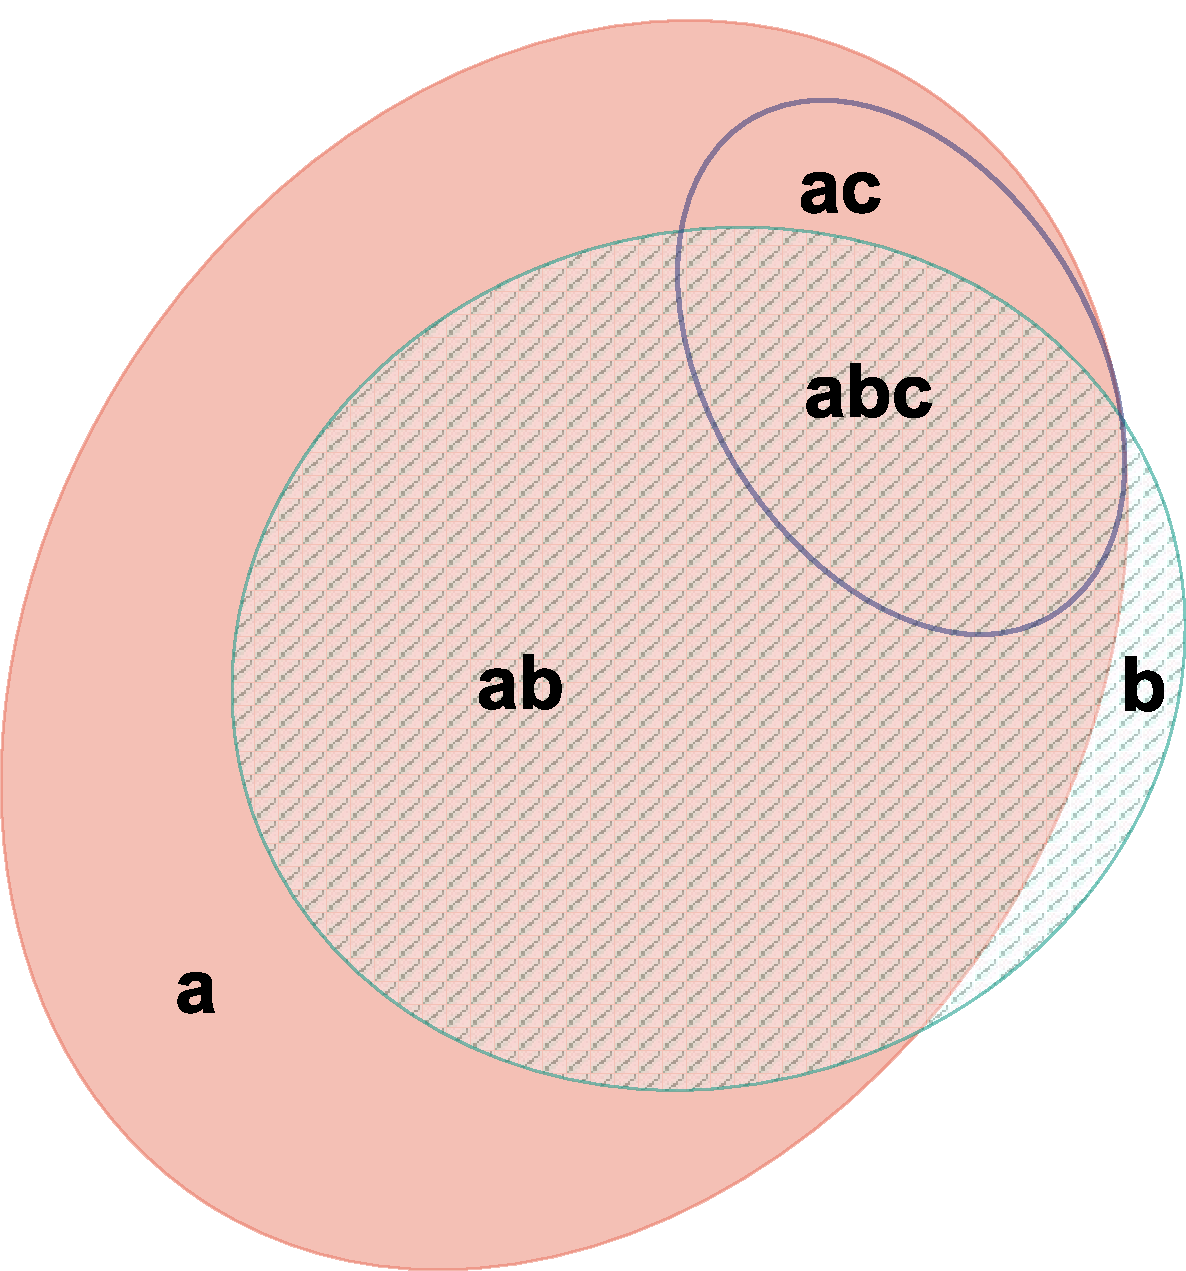
\includegraphics[height=.9\linewidth]{graphics//eulerape-lenz-a}
\subcaption{The diagram from \pkg{eulerAPE}.}
\end{subfigure}
\end{figure}

To conclude our case studies, we turn to a diagram
that was featured on the website of the author of
\pkg{venn.js}~\citep{Frederickson_2015a}. The diagram is based on the
\emph{Netflix Prize Dataset}\footnote{The dataset is no longer available
on this webpage, but has been archived at
\url{https://www.kaggle.com/netflix-inc/netflix-prize-data}
for those who are interested.}, from which the author
\begin{quote}
[...] picked 6 movies, kind of at random -- and then represented them using the
set of users that gave the movie a 5 star rating.
\end{quote}
The movies were \emph{Amelie, Pulp Fiction, Miss Congeniality, Armageddon, Rashomon,}
and \emph{Coyote Ugly}. The data only includes pairwise
relationships~(\cref{tab:netflix}).

\begin{table}
\caption{The data from the Netflix Prize dataset
used by \citet{Frederickson_2015a}. Each number indicates the number of
users who gave the corresponding movies a five-star rating.}
\label{tab:netflix}
\centering
\libertineTabular
\addtolength{\tabcolsep}{-2pt}
\small
\begin{tabular}{r|rrrrrr}
& \rot{Amelie} & \rot{Pulp Fiction} & \rot{Miss Congeniality} & \rot{Armageddon} & \rot{Rashomon} & \rot{Coyote Ugly}\\
\hline
Amelie            & 38,753 &&&&&\\
Pulp Fiction      & 15,197 & 70,153 &&&&\\
Miss Congeniality &  1,829 &  3,854 & 37,837 &&&\\
Armageddon        &  1,218 &  6,593 & 10,536 & 40,345 &&\\
Rashomon          &  2,087 &  2,799 &    132 &    143 & 6,209 &\\
Coyote Ugly       &    610 &  2,206 &  5,965 &  5,699 &    38 & 15,611
\end{tabular}
\end{table}



The fit from \pkg{eulerr} is marginally better than that of \pkg{venn.js}.
The stress and diagError of the \pkg{eulerr} diagram~(\cref{fig:netflix-eulerr})
are 0.003 and 0.014 respectively,
whilst the same figures are 0.004 and
0.015 for the \pkg{venn.js}
diagram~(\cref{fig:netflix-vennjs}).

\begin{figure*}[hbtp]
\begin{subfigure}[b]{.45\linewidth}
\centering
\begin{knitrout}\small
\definecolor{shadecolor}{rgb}{0.969, 0.969, 0.969}\color{fgcolor}

{\centering 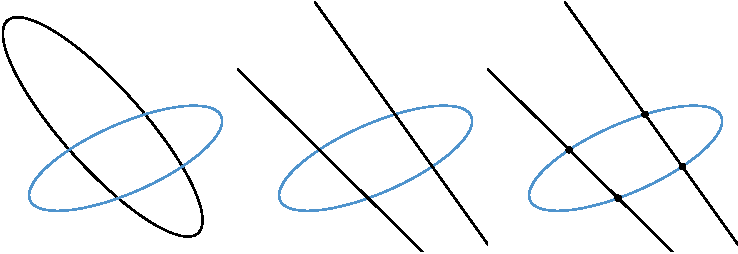
\includegraphics[width=\maxwidth]{figure/unnamed-chunk-2-1} 

}



\end{knitrout}
\subcaption{The fit from \pkg{eulerr} with a stress of
0.003 and diagError of 0.014.\label{fig:netflix-eulerr}}
\end{subfigure}\hfill%
\begin{subfigure}[b]{.45\linewidth}
\centering
\begin{knitrout}\small
\definecolor{shadecolor}{rgb}{0.969, 0.969, 0.969}\color{fgcolor}

{\centering 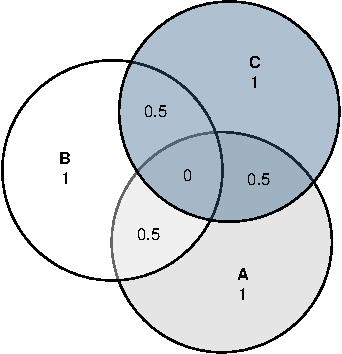
\includegraphics[width=\maxwidth]{figure/unnamed-chunk-3-1} 

}



\end{knitrout}
\subcaption{The fit from \pkg{venn.js} with a stress of
0.004 and diagError of 0.015.\label{fig:netflix-vennjs}}
\end{subfigure}
\caption{The Euler diagrams generated from the Netflix Prize data. The
difference in the two layouts primarily concern the placements of \emph{Rashomon}
and \emph{Miss Congeniality}.}
\label{fig:netflix}
\end{figure*}

\section{Consistency}
\label{sec:consistency}

To compare the consistency among \pkg{eulerr}, \pkg{venneuler}, \pkg{eulerAPE},
\pkg{venn.js}, and \pkg{Vennerable}, we generate random diagrams of circles and
ellipses (separately), compute their areas, and attempt to reproduce the original diagrams
using the various software. We restrict ourselves to
diagrams consisting of between three and eight shapes.

For the circles, we sample radii ($r_i$) and coordinates ($h_i$ and $k_i$) from
\begin{equation}
\begin{aligned}
h_i,k_i & \sim \mathcal{U}(0, 1)\\
r_i     & \sim \mathcal{U}(0.2, 0.6).
\end{aligned}
\label{eq:consistencyCircles}
\end{equation}
For the ellipses, we sample semiaxes ($a_i$ and $b_i$), coordinates
($h_i$ and $k_i$), and rotation axes ($\phi_i$) from
\begin{equation}
\begin{aligned}
h_i,k_i & \sim \mathcal{U}(0, 1)\\
r_i     & \sim \mathcal{U}(0.2, 0.6)\\
c_i     & \sim \mathcal{U}(0.5, 2)\\
a_i     & = c_ir_i\\
b_i     & = \frac{r_i}{c_i}\\
\phi_i  & \sim \mathcal{U}(0, \pi).
\end{aligned}
\label{eq:consistencyEllipses}
\end{equation}

Next, we compute the required areas, $\omega$~(\cref{def:omega})
and fit Euler diagrams using the aforementioned packages. Finally,
we compute and return diagError~\eqref{eq:diagError} and score each
diagram as a success if its diagError is lower than 0.01, that is,
if no portion of the diagram is one \emph{percentage point} off from that of the
input; note that this is always achievable since our input comes
from sampled diagrams.



For each number of shapes, $N=3,4,\dots,8$, we run the simulations until we have
achieved a 95\% confidence interval around $\hat{p}$, the proportion of
successful diagrams, no wider than 0, and for a minimum of 1,000 iterations. We
use the normal approximation interval,
\begin{equation}
\mathcal{I}(\hat{p})_{0.95} = \hat{p} \pm z_{0.95}\sqrt{\frac{\hat{p}(\hat{p}-1)}{n}}.
\label{eq:prop-ci}
\end{equation}
The procedure is formalized in~\cref{alg:consistency}. For circular diagrams,
\pkg{eulerr} outperforms \pkg{Vennerable} and \pkg{venneuler} in
consistency by considerable margin and is on par with \pkg{venn.js} and
\pkg{eulerAPE}~(\cref{fig:consistency}). \pkg{eulerr} and \pkg{eulerAPE} are
the only packages that successfully fits all of the circular diagrams (although
\pkg{eulerAPE} only accepts a subset of our three-set diagrams).
\pkg{venn.js} fails in 4 cases out of
6000.

\begin{algorithm}[  hbtp]
\caption{The algorithm used to simulate diagrams of circles or ellipses,
reverse-engineer set relationships,
and fit Euler diagrams to these relationships using the different software packages.
$\mathcal{I}(\hat{p})_{0.95}$ is the binomial proportion confidence
interval~\eqref{eq:prop-ci}.\label{alg:consistency}}
\begin{algorithmic}
\For{$N \gets 3:8$}
  \State $i, \text{successes} \gets 0$
  \Do
    \State $i \gets i + 1$
    \State $\alpha_i \gets \Call{random diagram}{}$
    \State $\omega_i \gets \Call{compute overlaps}{\alpha_i}$
    % \State $h_i,k_i \gets \mathcal{U}(0, 1)$
    % \State $r_i \gets \mathcal{U}(0.2, 0.6)$
    % \If{circle}
    %   \State $\omega_i \gets \Call{FindOverlaps}{h_i, k_i, r_i}$
    % \ElsIf{ellipse}
    %   \State $c_i      \gets \mathcal{U}(0.5, 2)$
    %   \State $a_i      \gets c_i r_i$
    %   \State $b_i      \gets r_i/c_i$
    %   \State $\phi_i   \gets \mathcal{U}(0, \pi)$
    %   \State $\omega_i \gets \Call{FindOverlaps}{h_i, k_i, a_i, b_i, \phi_i}$
    % \EndIf
    \ForAll{$j \gets$ software}
      \State $\hat{p}_j \gets \text{successes}_j/i$
      \If{$\mathcal{I}(\hat{p})_{0.95}$ is wider than 0.02 \Or $i \leq 1000$}
        \State $A_{i_j} \gets \Call{fit diagram}{\omega_i}$
        \If{$\Call{diagError}{A_{i_j}, \omega_i} < 0.01$}
          \State $\text{successes}_j \gets \text{successes}_j + 1$
        \EndIf
      \EndIf
    \EndFor
  \DoWhile{\All $\mathcal{I}(\hat{p})_{0.95}$ are wider than 0.02 \Or $i \leq 1000$}
\EndFor
\end{algorithmic}
\end{algorithm}

\begin{figure*}[bhtp]
\begin{knitrout}\small
\definecolor{shadecolor}{rgb}{0.969, 0.969, 0.969}\color{fgcolor}

{\centering \includegraphics[width=\maxwidth]{figure/consistency-1} 

}



\end{knitrout}
\caption{Proportions of successfully reproduced Euler diagrams from
set configurations based on sampled circular and elliptical diagrams generated from the
distributions in \eqref{eq:consistencyCircles} and \eqref{eq:consistencyEllipses}.
The results are based on at least 1000 iterations for each
software package and number of sets and have at most a 0.02-wide
symmetric 0.95\% confidence interval around the displayed point estimate. A
success is defined as a diagram with a diagError~\eqref{eq:diagError} below
0.01.}
\label{fig:consistency}
\end{figure*}

For ellipses of three shapes, \pkg{eulerr} successfully fits all diagrams
whilst \pkg{eulerAPE} fails in
6
cases out of 1000.

For ellipses of four or more sets---which only \pkg{eulerr} accepts---the
consistency drops for each additional set, from 78\%
at four sets to
38\% at eight sets. \pkg{Vennerable}, which
is only able to produce three-set diagrams, only produces accurate diagrams for
7\% of the random layouts and moreover
fails with an error in 6 cases.

\section{Accuracy}
\label{sec:accuracy}

In \cref{sec:consistency}, we assessed the efficacy in reproducing diagrams
with exact, albeit unknown, solutions. Reality, however, often presents us with
relationships that lack such exact solutions. Yet, when there is no
exact solution, one might still exist that is \emph{good enough},
which we naturally want our model to find.

To assess the accuracy in producing diagrams for which there might not be an
exact fit,
we generate random set relationships, fiting Euler diagrams to each using the
software under study. For each $N=3,4,\dots,8$ sets, we initialize
$N$-set combinations with all items set to 0. For every set relationship, we pick $N$
elements from the relationship at random---making sure that each set is selected
at least once---and assign to each a number generated
from $\mathcal{U}(\epsilon, 1)$, where $\epsilon$ is defined as the square root
of the current machine's smallest
representable difference between one and the smallest value greater than
one\footnote{The R-code used to generate this $\epsilon$ is
\code{sqrt(.Machine\$double.eps)}}. Next, we draw a sample of a random subset of
the remaining $2^N-1-N$ set intersections and assign to them a number from
$\mathcal{U}(\epsilon, 1)$ as before.

We run our simulations for a minimum of 1,000 iterations and until we achieve
a 95\% confidence interval around the mean diagError no wider than 0.02.
The confidence level used is based on the
$t$-distribution,
\begin{equation}
\mathcal{I}(\bar{x})_{0.95} = \bar{x} \pm t_{0.95}\frac{s}{\sqrt{n}},
\label{eq:mean-ci}
\end{equation}
where \[s = \sqrt{\frac{1}{N-1}\sum_{i=1}^n (x - \bar{x})^2}.\]
The procedure is formalized in~\cref{alg:accuracy}.

\begin{algorithm}[hbtp]
\caption{The algorithm used to simulate and fit random set relationships to assess
the accuracy of the various software we are studying. $\mathcal{I}(\bar{x})_{0.95}$
is the 95\% confidence interval around the mean diagError~\eqref{eq:mean-ci},
$F$ denotes a set, and
$\epsilon$ is the square root of the
difference between 1 and the least value greater than 1 on our machine.\label{alg:accuracy}}
\begin{algorithmic}
\For{$N \gets 3:8$}
  \State $i \gets 0$
  \Do
    \State $i \gets i + 1$
    %\State $\omega_i$ so that all $N$ sets are represented
    %\State $\omega_i \gets \{\omega_{i_1},\omega_{i_2},\dots,\omega_{i_{2^N-1}} \}$
    \For{$k \gets 1:N$}
      \State random element in $\{\omega_i : \omega_i \cap F_k \neq \emptyset\} \gets \mathcal{U}(\epsilon, 1)$
      %\State $\omega_{i_k} \gets \mathcal{U}(\epsilon, 1)$
    \EndFor
    % \State $\Omega_i \gets \{\omega_i : \omega_i = 0\}$
    % \For{$l \gets 1,2,\dots$}
    %   \State $w_l \gets \text{Bernoulli}(0.5)$
    %   \If{$w_l$}
    %     \State $\Omega_{i_l} \gets \mathcal{U}(\epsilon, 1)$
    %   \EndIf
    % \EndFor
    \ForAll{$j \gets$ software packages}
      \State $A_{j_i} \gets \Call{fit diagram}{\omega_i}$
      \State $x_{j_i} \gets \Call{diagError}{A_{j_i},\omega_i}$
    \EndFor
  \DoWhile{\All $\mathcal{I}(\bar{x})_{0.95}$ are wider than 0.02 \Or $i \leq 1000$}
\EndFor
\end{algorithmic}
\end{algorithm}

However, given that neither \pkg{Vennerable} nor \pkg{eulerAPE} are capable
of fitting Euler diagrams that feature subset or disjoint relationships, and
because fully intersecting diagrams are more difficult to fit---at least
with circles---we run a separate treatment
in which we modify~\cref{alg:accuracy} so that every intersection
is initialized to a value in $\mathcal{U}(\epsilon, 1)$.



From the results generated via \cref{alg:accuracy}, we can
surmise that \pkg{eulerr}'s elliptical diagrams achieve the lowest median stress and
diagError~(\cref{fig:accuracy}) for all set sizes, although the difference is
relatively more pronounced for set sizes three and four.

\begin{figure*}[hbtp]
\begin{knitrout}\small
\definecolor{shadecolor}{rgb}{0.969, 0.969, 0.969}\color{fgcolor}

{\centering \includegraphics[width=\maxwidth]{figure/accuracy-1} 

}



\end{knitrout}
\caption{Tukey box plots of Euler diagrams based on set relationships that may
or may not have perfect solutions, generated from~\eqref{eq:consistencyEllipses}.\label{fig:accuracy}}
\end{figure*}

We also find that among the algorithms that fit circular Euler diagrams,
\pkg{eulerr} offers the lowest median stress across all the sizes of set
relationships. For diagError, however, \pkg{venn.js} produces diagrams with the
least loss for three sets, whilst \pkg{eulerr} scores better for all the remaining set sizes,
for which \pkg{venn.js} is moreover outdone by \pkg{venneuler}.



Looking at the results from the simulation of three-set relationships with
all intersections present~(\cref{fig:accuracy-int}), \pkg{eulerr} still
produces the most accurate diagrams provided that we use ellipses---both in
terms of stress and diagError. The
difference next to \pkg{eulerAPE} is neglible, however, with differences
below $10^{-7}$.

\begin{figure}[hbtp]
\caption{Tukey box plots of diagError and stress for Euler diagrams
based on set relationships of three sets with every
intersection present.\label{fig:accuracy-int}}
\begin{knitrout}\small
\definecolor{shadecolor}{rgb}{0.969, 0.969, 0.969}\color{fgcolor}

{\centering \includegraphics[width=\maxwidth]{figure/accuracy-int-1} 

}



\end{knitrout}
\end{figure}

For circular diagrams, \pkg{venn.js} achieves the lowest median diagError at
0.044, followed by \pkg{venneuler} at 0.048,
\pkg{eulerr} at 0.055, \pkg{eulerAPE} at 0.067,
and \pkg{Vennerable} at 0.1. As for stress, however, the order is
partially reversed with respective stress values at
0.022, 0.035, 0.044, 0.08,
0.159 for
\pkg{eulerr}, \pkg{venneuler}, \pkg{venn.js}, \pkg{eulerAPE}, and \pkg{Vennerable}
respectively.

\section{Performance}
\label{sec:performance}

Using the same procedure as in \cref{alg:accuracy}, we generate random set
relationships and measure the time it takes for each software package to form a
diagram from the input. We use \pkg{microbenchmark}~\citep{Ooms_2017} for the benchmarks,
which randomizes the order in which the packages are called between trials.
Because neither the current version of \pkg{venn.js}, nor any version of \pkg{eulerAPE},
have been implemented in R, we omit these packages from the
performance benchmarks.



\pkg{eulerr} is faster for circular diagrams up to and including seven
sets~(\cref{fig:performance}), after which \pkg{venneuler} catches
up and subsequently outperforms \pkg{eulerr} for eight-set relationships. For a three-set diagram,
for instance, \pkg{eulerr} takes a median of
0.007
seconds to find a fit, whilst \pkg{venneuler} takes 0.414
seconds, and \pkg{Vennerable} 0.056
seconds. For eight sets, meanwhile, \pkg{eulerr} takes
2.68
seconds and \pkg{venneuler} 2.059.

The computation time for the elliptical
diagrams from \pkg{eulerr} generally vary more but are still, on average,
faster than \pkg{venneuler} for up to five sets---albeit with the exception
of diagrams of three sets, where the resulting bimodal distribution is a
consequence of the time-consuming
last-ditch optimizer (\cref{sec:last-ditch}) that is activated by default
if the fit is not error-free after the final optimizer.

\begin{figure*}[hbtp]
\begin{knitrout}\small
\definecolor{shadecolor}{rgb}{0.969, 0.969, 0.969}\color{fgcolor}

{\centering \includegraphics[width=\maxwidth]{figure/performance-1} 

}



\end{knitrout}
\caption{Violin plot of the performance of \pkg{eulerr}, \pkg{venneuler}, and \pkg{Vennerable} on
random set relationships of three to eight sets. The density smoother is that of \citet{Sheather_1991}.}
\label{fig:performance}
\end{figure*}

\chapter{Discussion}
\label{ch:discussion}

In this thesis, we have presented a novel method for generating elliptical Euler diagrams
for any number of sets. We have shown that the package
is both more consistent and accurate than the other packages analyzed as well as
faster for up to seven sets.

\pkg{eulerr} reproduced all the circular diagrams
generated in \cref{sec:consistency} within our stipulated margin of error.
No other package managed this task, although the failing diagrams of both
\pkg{eulerAPE} and \pkg{venn.js} numbered in the single digits.
\pkg{venneuler}, in contrast, was not able to adequately
reproduce 57\%
of these diagrams, which, however, was still
better than the results on a previous
test~\citep{Frederickson_2015b}.

Some of the examined set relationships feature disjoint or subset
relationships, which \pkg{venneuler} have problems fitting on account of its
initial optimizer. As we discussed in \cref{sec:background},
\pkg{eulerr}, \pkg{venn.js}, and \pkg{venneuler} all use multi-dimensional scaling for
their initial diagram. \pkg{venneuler}, however, unnecessarily restricts the
locations of disjoint and subset circles. Given, for instance, two disjoint
sets, the algorithm will attempt to place them tangent to one another; otherwise,
the optimizer will report loss. Likewise, for a subset
relationship, \pkg{venneuler} tries to place the smaller circle at the exact
midpoint of the enclosing shape.

For the fit to be accurate, however, those restrictions are pointless as long as
the sets remain disjoint or subset.
For \pkg{venneuler}, this becomes problematic because the required positions might interfere
with space that could be used by other sets to improve the fit. The
constrained multi-dimensional scaling method in \pkg{venn.js} and
\pkg{eulerr} circumvents this by
assigning a loss and gradient of zero when the pairwise set intersection
\emph{and} the candidate circles are disjoint or subset. This makes it easier
for the starting layout to find a good initial layout.

Another reason for the mediocre results of \pkg{venneuler} could be both that the optimizer
terminates prematurely in case the relative reduction in stress is considered negligible
between iterations \emph{or} that the number of iterations is too low.

\pkg{eulerr} managed to also reproduce all of the elliptical
three-set diagrams perfectly but failed for an increasing number of cases as we
added sets to our input.
For three-set diagrams, \pkg{eulerr} employs a rigorous last-ditch
optimizer in case the fit it not adequate after the first step of
the final optimization procedure. This step is
time-consuming (as we saw in \cref{sec:performance}), but if activated
would yield better results also for sets of more than three shapes.

The elliptical diagrams from \pkg{eulerr} are more accuracte for
set relationships that might lack exact solutions compared with the
other packages in this thesis, although the difference next to \pkg{eulerAPE}
is slight. Elliptical Euler diagrams are more successful since they
allow two additional degrees of freedom for each set, that is,
rotation and stretching. The marginal gains
are greatest for three sets and diminishes as we add more sets. This is what we
expect: complicated inputs require
complicated models and there are many set configurations that even elliptical Euler
diagrams cannot support---consider, for instance, the complicated geometry of the
Venn diagram in \cref{fig:edwards} that is required to represent
all the intersections between six sets.

\begin{marginfigure}
\begin{knitrout}\small
\definecolor{shadecolor}{rgb}{0.969, 0.969, 0.969}\color{fgcolor}

{\centering \includegraphics[width=\maxwidth]{figure/battlement-1} 

}



\end{knitrout}
\caption{A six-set Venn diagram using Edward's method~\cite{Edwards_2014};
this diagram was generated with \pkg{Vennerable}.}
\label{fig:edwards}
\end{marginfigure}

Considering only circular Euler diagrams, \pkg{eulerr} remains the best
choice for both diagError and stress in all cases except for three-set
diagrams, where it ranks best in terms of stress but not
diagError, which \pkg{venn.js} scores best on. It might be appropriate to note,
however, that \pkg{eulerr}, \pkg{venneuler}, and \pkg{venn.js} all
try to minimize the residual sums of squares in one way or
another---\emph{not} diagError. In essence, this means that the lower
diagError from \pkg{venn.js}, regardless of whether it is desired, is
not a sign that the algorithm performed as intended, particularly
not when stress is considered as well\footnote{Stress, on the other
hand, \emph{is} directly related to the residual sums of squares.}.

Surprisingly, given the results
in \cref{sec:consistency}, \pkg{venn.js} performs worse than \pkg{venneuler}
in all of the remaining cases. We can only speculate as to reasons for this,
but it is possible that the Nelder--Mead variant used in \pkg{venn.js}
chokes on the more complicated layouts; indeed, this was our experience when
designing \pkg{eulerr}, which at one point featured a version of the same
optimizer. In our case,
\code{nlm()} from the \pkg{stats} package was found to be superior.

In contrast to \pkg{eulerAPE}'s elliptical diagrams, its circular ones
performed worse than all other packages save for \pkg{Vennerable}. This result likely
stems from the particular loss function used in \pkg{eulerAPE}, which
prohibits empty overlaps in the diagram---often at the expense of the overall fit. The
author's argue that this function drives the optimizer away from local
minima~\cite{Micallef_2014a}, but we could not find any such issues with
\pkg{eulerr}. On the other hand, this feature of \pkg{eulerAPE} might
be desired by those who prioritize the nominal\footnote{Nominal in the sense
that each relationship in the input is also represented in the diagram.}, rather than
proportional, representativeness of the diagram.

Performance-wise, \pkg{eulerr} is faster than both \pkg{Vennerable} and
\pkg{venneuler} for up to seven sets. One reason for this is likely the implementation
in \proglang{C++} and use of the Armadillo library~\citep{Sanderson_2016}
provided by the interfaces \pkg{Rcpp}~\citep{Eddelbuettel_2011} and
\pkg{RcppArmadillo}~\citep{Eddelbuettel_2014}.
Another reason---possibly the foremost---comes from the exact-area algorithm that
involves less work than the quadtrees of \pkg{venneuler} with few sets.

Paradoxically, this is also why the performance of \pkg{eulerr}
suffers as the number of sets increase. In essence, we must examine every
possible intersection when computing the areas. For eight sets, for instance,
this means investigating $2^8-1 = 255$ intersections. Asymptotically, the
algorithm thus converges in $\mathcal{O}(2^n)$ time. \citet{Wilkinson_2012},
meanwhile, report convergence for \pkg{venneuler} in $\mathcal{O}(n)$ time, which
there indeed is evidence of in \cref{fig:performance}. As a result, the
computational demand of complicated set configurations make fitting difficult diagrams
with \pkg{eulerr} prohibitive where speed is a concern. On the other hand,
Euler diagrams seldom make sense for such complicated set relationships---only rarely will they
conform to an adequate fit. Nevertheless, future versions of this algorithm should
consider implementing approximate area-calculations when the number of sets is
large to cater to the, albeit few, instances where a Euler diagram is
appropriate.

Fitting diagrams is substantially harder with ellipses than with circles.
There are many more local minima that might hobble our optimizer
and since our initial configuration only
considers circles, such minima cannot reliably be avoided before the final
optimization step. And because we default to a local optimizer in this final step,
it is not uncommon that we terminate before finding the global minimum.
The last-ditch optimizer
battles such minima with brute force: it tries a vast number of permutations
and uses the previous fits (initial and semi-final) only to set up
constraints for the algorithm. The downside to using this algorithm is that it,
in contrast to human beings, does not favor circles over ellipses, which means
that we might get elliptical diagrams when circular ones would do. Future
efforts in this field should consider penalization, or similar techniques,
in order to promote user-friendly diagrams.

\section{Conclusion}
\label{sec:conclusion}

In all of the scenarios examined in this thesis,
\pkg{eulerr}'s elliptical Euler diagrams offer solutions with the least error
among all of the packages
tested. For three sets, \pkg{eulerr}'s accuracy is equalled only by the elliptical diagrams from
\pkg{eulerAPE}, which, however, impose restrictions that
\pkg{eulerr} do not, namely, that there be no disjoint or subset relationships.
% In addition, \pkg{eulerr} offers considerable control over the visual output,
% which is levied via the \pkg{lattice} package~\citep{Sarkar_2008} for R.

\pkg{eulerAPE}'s restriction to three sets is discussed by the authors of the
package, who motivate this limitation with the propensity of Euler diagrams with
more sets to lack adequate solutions and that their complexity make
implementations difficult~\citep{Micallef_2013}. Whilst it is true that
inputs with more than three sets do not always reduce to adequate Euler diagrams,
it is our stance that those that \emph{do}, warrant a software implementation that
enables users to find them, given that Euler diagrams are intuitive
visualizations that are easily grasped by most viewers.

The foremost shortcoming of \pkg{eulerr} is its failure to consistently
find optimal elliptical diagrams, which is evident in \cref{sec:consistency},
wherein a portion of the sampled diagrams are not refit adequately,
implying that the accuracy (see \cref{sec:accuracy})
must have potential to improve. This problem is not intractable and we
believe it could be overcome either by
\begin{itemize}
\item relying on brute-force global optimizers that thoroughly examine
the search space and attempt to optimize---possibly parallelize---these routines
to make complex diagrams fit with reasonable speed, or by
\item designing an algorithm for the initial configuration that works
specifically for ellipses and avoids local minima ahead of final
optimization.
\end{itemize}
Whichever direction future research takes, we believe that the advances
presented in this thesis serves as another step in the direction towards more
accurate Euler diagrams.

\begin{fullwidth}
\part*{Appendices}
\end{fullwidth}
\appendix
\chapter{Visualization}
\label{ap:visualization}

Once we have ascertained that our Euler diagram fits well, we can turn to
visualizing the solution. For this purpose, \pkg{eulerr} leverages the
\pkg{Lattice} graphics system~\citep{Sarkar_2008} for R to offer intuitive and
granular control over the output.

Plotting the ellipses is straightforward using the parametrization of a rotated
ellipse,
%
\begin{equation*}
\begin{bmatrix}
  x \\ y
\end{bmatrix} =
\begin{bmatrix}
  h + a \cos{\theta} \\
  k + b \sin{\theta}
\end{bmatrix},\quad \text{where } \theta \in [0, 2\pi],\, a,b>0.
\end{equation*}
%
Most users will also prefer to label the ellipses and their intersections
with text and this, however, is considerably more involved.

\section{Labeling}
\label{sec:labeling}

Labeling the ellipses is complicated since the shapes of the intersections
often are irregular, lacking well-defined centers; we know of no analytical
solution to this problem. As usual, however, the next-best option turns out to
be a numerical one. First, we locate a point that is inside the required region
by spreading points across the discs involved in the set intersection. To
distribute the points, we use a modification of
\emph{Vogel's method}~\citep{Arthur_2015,Vogel_1979} adapted to ellipses.
Vogel's method spreads points across a disc using
\begin{equation}
p_k =
\begin{bmatrix}
  \rho_k \\
  \theta_k
\end{bmatrix} =
\begin{bmatrix}
  r \sqrt{\frac{k}{n}}\\
  \pi (3 - \sqrt{5})(k - 1)
\end{bmatrix}\quad\text{for } k = 1, 2,\dots, n.
\label{eq:vogel}
\end{equation}
In our modification, we scale, rotate, and translate the points formed
in~\eqref{eq:vogel} to match the candidate ellipse. We rely, as before, on
projective geometry to carry out the transformations in one go:
\[
p' =
\begin{bmatrix}
  x' \\
  y' \\
  1
\end{bmatrix} =
\begin{bmatrix}
  1 & 0 & h \\
  0 & 1 & k \\
  0 & 0 & 1
\end{bmatrix}
\begin{bmatrix}
  \cos{\phi}  & \sin{\phi} & 0 \\
  -\sin{\phi} & \cos{\phi} & 0\\
  0           & 0          & 1
\end{bmatrix}
\begin{bmatrix}
  a & 0 & 0 \\
  0 & b & 0 \\
  0 & 0 & 1
\end{bmatrix}
\begin{bmatrix}
  \hat{x} \\
  \hat{y} \\
  1
\end{bmatrix},
\]
where $h,k$ translates, $\phi$ rotates, and
$a,b$ stretches the ellipse.

After we spread our points throughout the ellipse and find a point, $p'_i$, that
is contained in our desired intersection, we proceed to optimize its position
numerically. The position we are looking for is that which maximizes the
distance to the closest ellipse in our diagram to provide as much margin as
possible for the label. This is a maximization problem with a loss function equal to
\begin{equation}
\mathcal{L}(x,y) = \min_{i=1,2,\dots,N} f(x,y,h_i,k_i,a_i,b_i,\phi_i)
\label{eq:lossDist}
\end{equation}
where $f$ is the function that determines the distance from a point ($x,y$) to
the ellipse defined by $h,k,a,b$ and $\phi$.

Similarly to fitting Euler diagrams in the general case, there appears to be no
analytical solution to computing the distance from a point to an ellipse. The
numerical solution we use has been described by~\citet{Eberly_2016a} and
involves solving the roots to a quartic polynomial via a robust
bisection optimizer.

To optimize the location of the label, we employ a version of the
\emph{Nelder--Mead method}~\citep{Nelder_1965}, which has been translated from
a \proglang{Matlab} code by \citet{Kelley_1999} and adapted for \pkg{eulerr} to
ensure that it converges quickly and that the simplex remains within the
intersection boundaries (since we want the local maximum). The method is
visualized in~\cref{fig:vogel}.
\begin{marginfigure}
\begin{knitrout}\small
\definecolor{shadecolor}{rgb}{0.969, 0.969, 0.969}\color{fgcolor}

{\centering \includegraphics[width=\maxwidth]{figure/vogel-1} 
\includegraphics[width=\maxwidth]{figure/vogel-2} 
\includegraphics[width=\maxwidth]{figure/vogel-3} 

}



\end{knitrout}
\caption{The method eulerr uses to locate an optimal position for a label in
three steps from top to bottom: first, we spread sample points on one of the
ellipses and pick one inside the intersection of interest, then we begin moving
it numerically, and finally place our label.}
\label{fig:vogel}
\end{marginfigure}

\section{Aesthetics}
\label{sec:aesthetics}

Euler diagrams display both quantitative and qualitative data. The quantitative
aspect is the quantities or sizes of the sets depicted in the diagram and is
visualized by the relative sizes, and possibly the labels, of the areas of the
shapes---this is the main focus of this paper. The qualitative aspects,
meanwhile, consist of the mapping of each set to some quality or category, such
as having a certain gene or not. In the diagram, these qualities can be
separated through any of the following aesthetics:
%
\begin{itemize}
\item color,
\item border type,
\item text labelling,
\item transperancy,
\item patterns,
\end{itemize}
%
or a combination of these. The main purpose of these aethetics is to separate
out the different ellipses so that the audience may interpret the diagram with
ease and clarity.

Among these aesthetics, the best choice (from a viewer perspective) appears to
be color~\citep{Blake_2016}, which provides useful information without
extraneous chart junk~\citep{Tufte_2001}. The issue with color, however, is that
it cannot be perceived perfectly by all---8\% of men and 0.4\% of women in
European Caucasian countries, for instance, suffer the most common form,
red--green color deficiency~\cite{Birch_2012}. Moreover, color
is often printed at a premium in scientific publications and adds no information
to a diagram of two shapes.

For these reasons, \pkg{eulerr} defaults to distinguishing ellipses with color
using a color palette generated via the R package
\pkg{qualpalr}~\citep{Larsson_2016}, which automatically generates qualitative
color palettes based on a perceptual model of color vision that optionally
caters to color vision deficiency. This palette has been manually modified
to fullfil our other objectives of avoiding using colors for two
sets. The first eight colors of the pallete are visualized in
\cref{fig:colorexample}.

\begin{figure}[htbp]
\caption{The eight first colors of the default color palette.\label{fig:colorexample}}
\begin{knitrout}\small
\definecolor{shadecolor}{rgb}{0.969, 0.969, 0.969}\color{fgcolor}

{\centering \includegraphics[width=\maxwidth]{figure/colorexamle-1} 

}



\end{knitrout}
\end{figure}

\section{Normalizing dispered layouts}
\label{sec:layout}

If there are disjoint clusters of ellipses, the optimizer will often
spread these out more than is necessary, wasting space in our diagram. To
tackle this, we
use a SKYLINE-BL rectangle packing algorithm~\citep{Jylaenki_2010}
designed specifically for \pkg{eulerr}. In it, we surround each ellipse cluster
with a bounding box, pack these boxes into a bin of appropriate size and
aspect ratio, and adjust the coordinates of the ellipses in the clusters to
compact our diagram. As a bonus, this increases the chance of having
similar layouts for different function calls.

\chapter{Usage}\label{ch:usage}

\code{euler()} and \code{plot()} are the only functions that users of
\pkg{eulerr} need concern themselves with. In \cref{sec:input}, we described
the various forms of input that the function can be supplied with. Using the
first form, we will showcase how a Euler diagram is fit. For this example,
we use a diagram from a publication by \citet{Junta_2009} that was also
tackled by \citet{Wilkinson_2012}. We load the package,
specify our diagram, and fit it using \code{euler()} as follows.

\begin{knitrout}\small
\definecolor{shadecolor}{rgb}{0.969, 0.969, 0.969}\color{fgcolor}\begin{kframe}
\begin{alltt}
\hlkwd{library}\hlstd{(eulerr)}
\hlstd{junta_2009} \hlkwb{<-} \hlkwd{c}\hlstd{(}\hlstr{"SE"} \hlstd{=} \hlnum{13}\hlstd{,} \hlstr{"Treat"} \hlstd{=} \hlnum{28}\hlstd{,} \hlstr{"Anti-CCP"} \hlstd{=} \hlnum{101}\hlstd{,}
                \hlstr{"DAS28"} \hlstd{=} \hlnum{91}\hlstd{,} \hlstr{"SE&Treat"} \hlstd{=} \hlnum{1}\hlstd{,} \hlstr{"SE&DAS28"} \hlstd{=} \hlnum{14}\hlstd{,}
                \hlstr{"Treat&Anti-CCP"} \hlstd{=} \hlnum{6}\hlstd{,} \hlstr{"SE&Anti-CCP&DAS28"} \hlstd{=} \hlnum{1}\hlstd{)}
\hlstd{fit1} \hlkwb{<-} \hlkwd{euler}\hlstd{(junta_2009)}
\end{alltt}
\end{kframe}
\end{knitrout}

Printing the results provides a summary of the fit, including the stress
and diagError metrics that were introduced in~\cref{sec:gof}.

\begin{knitrout}\small
\definecolor{shadecolor}{rgb}{0.969, 0.969, 0.969}\color{fgcolor}\begin{kframe}
\begin{alltt}
\hlstd{fit1} \hlcom{# or equivalently print(fit1)}
\end{alltt}
\begin{verbatim}
##                         original fitted residuals regionError
## SE                            13 12.780     0.220       0.000
## Treat                         28 27.525     0.475       0.000
## Anti-CCP                     101 99.287     1.713       0.002
## DAS28                         91 89.457     1.543       0.001
## SE&Treat                       1  0.983     0.017       0.000
## SE&Anti-CCP                    0  0.000     0.000       0.000
## SE&DAS28                      14 13.763     0.237       0.000
## Treat&Anti-CCP                 6  5.898     0.102       0.000
## Treat&DAS28                    0  0.000     0.000       0.000
## Anti-CCP&DAS28                 0  0.000     0.000       0.000
## SE&Treat&Anti-CCP              0  0.000     0.000       0.000
## SE&Treat&DAS28                 0  0.000     0.000       0.000
## SE&Anti-CCP&DAS28              1  0.000     1.000       0.004
## Treat&Anti-CCP&DAS28           0  0.000     0.000       0.000
## SE&Treat&Anti-CCP&DAS28        0  0.000     0.000       0.000
## 
## diagError: 0.004 
## stress:    0
\end{verbatim}
\end{kframe}
\end{knitrout}

The fit is more or less equivalent to that of
\pkg{venneuler}~\citep{Wilkinson_2012}. There \emph{is} an error but it is
small at a diagError of 0.004. We could, however, try to
improve the fit using ellipses:

\begin{knitrout}\small
\definecolor{shadecolor}{rgb}{0.969, 0.969, 0.969}\color{fgcolor}\begin{kframe}
\begin{alltt}
\hlcom{# Fit the data using ellipses instead}
\hlstd{fit2} \hlkwb{<-} \hlkwd{euler}\hlstd{(junta_2009,} \hlkwc{shape} \hlstd{=} \hlstr{"ellipse"}\hlstd{)}

\hlcom{# Compare the fits on diagerror}
\hlstd{fit1}\hlopt{$}\hlstd{diagError} \hlopt{-} \hlstd{fit2}\hlopt{$}\hlstd{diagError}
\end{alltt}
\begin{verbatim}
## [1] 0
\end{verbatim}
\end{kframe}
\end{knitrout}

Comparing the two fits in diagError, however, shows that we have not bettered
the fit in any meaningful way. Our next goal is to visualize the layout, which
we do both using the default options and by customizing the fit, adding
quantities, replacing the sets' labels with a key, removing lines, and changing the
fills~(\cref{fig:plotting}) using the \pkg{RColorBrewer} package~\citep{Neuwirth_2014}.

\begin{knitrout}\small
\definecolor{shadecolor}{rgb}{0.969, 0.969, 0.969}\color{fgcolor}\begin{kframe}
\begin{alltt}
\hlstd{p1} \hlkwb{<-} \hlkwd{plot}\hlstd{(fit1)}
\hlstd{p2} \hlkwb{<-} \hlkwd{plot}\hlstd{(fit1,}
           \hlkwc{quantities} \hlstd{=} \hlkwd{list}\hlstd{(}\hlkwc{fontface} \hlstd{=} \hlnum{3}\hlstd{),}
           \hlkwc{fill} \hlstd{= RColorBrewer}\hlopt{::}\hlkwd{brewer.pal}\hlstd{(}\hlnum{4}\hlstd{,} \hlstr{"Set2"}\hlstd{),}
           \hlkwc{border} \hlstd{=} \hlstr{"transparent"}\hlstd{,}
           \hlkwc{auto.key} \hlstd{=} \hlkwd{list}\hlstd{(}\hlkwc{space} \hlstd{=} \hlstr{"right"}\hlstd{))} \hlcom{# key on the right}
\end{alltt}
\end{kframe}
\end{knitrout}

\begin{figure}[hbtp]
\caption{The same fit visualized in two distinct ways.\label{fig:plotting}}
\begin{subfigure}[b]{.4\linewidth}
\begin{knitrout}\small
\definecolor{shadecolor}{rgb}{0.969, 0.969, 0.969}\color{fgcolor}

{\centering \includegraphics[width=\maxwidth]{figure/twofits1-1} 

}



\end{knitrout}
\subcaption{The default settings.}
\end{subfigure}%
\begin{subfigure}[b]{.6\linewidth}
\begin{knitrout}\small
\definecolor{shadecolor}{rgb}{0.969, 0.969, 0.969}\color{fgcolor}

{\centering \includegraphics[width=\maxwidth]{figure/twofits2-1} 

}



\end{knitrout}
\subcaption{Custom plot settings.}
\end{subfigure}
\end{figure}

\begin{fullwidth}
\bibliography{eulerr}
\bibliographystyle{unsrtnat}
\end{fullwidth}

\end{document}
